\documentclass[aspectratio=169, 10pt]{beamer}

%% ─── PACKAGES ───────────────────────────────────────────────────────────────
\usepackage[french]{babel}
\usepackage[utf8]{inputenc}
\usepackage[T1]{fontenc}
\usepackage{lmodern}
\usepackage{tikz}
\usepackage{pgfplots}
\pgfplotsset{compat=1.18}
\usepackage{fontawesome5}
\usepackage{booktabs}
\usepackage{graphicx}
\usepackage{xcolor}
\usepackage{array}
\usepackage{colortbl}
\usepackage{multirow}

%% ─── COULEURS ────────────────────────────────────────────────────────────────
\definecolor{acBlue}{RGB}{0, 56, 130}
\definecolor{acLightBlue}{RGB}{0, 120, 215}
\definecolor{acGold}{RGB}{218, 165, 32}
\definecolor{acGray}{RGB}{245, 246, 248}
\definecolor{acRed}{RGB}{192, 0, 0}
\definecolor{acGreen}{RGB}{0, 130, 80}
\definecolor{acDarkGray}{RGB}{80, 80, 80}

%% ─── THÈME BEAMER ────────────────────────────────────────────────────────────
\usetheme{default}
\usecolortheme{default}
\setbeamertemplate{navigation symbols}{}
\setbeamertemplate{itemize items}{\color{acLightBlue}\faChevronRight}
\setbeamertemplate{itemize subitem}{\color{acGold}\faMinus}

%% Couleurs globales
\setbeamercolor{frametitle}{bg=acBlue, fg=white}
\setbeamercolor{title}{fg=white}
\setbeamercolor{subtitle}{fg=acGold}
\setbeamercolor{author}{fg=white}
\setbeamercolor{date}{fg=white}
\setbeamercolor{normal text}{fg=acDarkGray}
\setbeamercolor{structure}{fg=acBlue}
\setbeamercolor{block title}{bg=acBlue, fg=white}
\setbeamercolor{block body}{bg=acGray, fg=acDarkGray}
\setbeamercolor{alerted text}{fg=acRed}
\setbeamercolor{example text}{fg=acGreen}

%% Frametitle design
\setbeamertemplate{frametitle}{%
  \vspace{0.15cm}
  \begin{beamercolorbox}[wd=\paperwidth, ht=0.7cm, dp=0.2cm, leftskip=0.4cm]{frametitle}
    \usebeamerfont{frametitle}\insertframetitle
    \ifx\insertframesubtitle\@empty\else
      \hfill{\color{acGold}\small\textit{\insertframesubtitle}}
    \fi
  \end{beamercolorbox}%
}

%% Footline
\setbeamertemplate{footline}{%
  \begin{beamercolorbox}[wd=\paperwidth, ht=0.4cm, dp=0.15cm]{footline}
    \begin{tikzpicture}[remember picture, overlay]
      \fill[acBlue] (0,0) rectangle (\paperwidth, 0.55cm);
      \node[anchor=west, text=white, font=\tiny] at (0.3cm, 0.275cm)
        {automaticCHECK — Sara Houéfa ADJAHO};
      \node[anchor=east, text=acGold, font=\tiny\bfseries] at (\paperwidth-0.3cm, 0.275cm)
        {\insertframenumber\,/\,\inserttotalframenumber};
    \end{tikzpicture}
  \end{beamercolorbox}%
}

%% Headline vide
\setbeamertemplate{headline}{}

%% ─── COMMANDES UTILITAIRES ───────────────────────────────────────────────────
\newcommand{\chiffrecle}[2]{%
  \begin{beamercolorbox}[rounded=true, wd=3.2cm, center, sep=0.25cm]{block title}
    {\Large\bfseries #1}\\[0.1cm]
    {\scriptsize #2}
  \end{beamercolorbox}%
}

\newcommand{\carteinfo}[3]{%
  \begin{tikzpicture}
    \fill[#1, rounded corners=4pt] (0,0) rectangle (3.6cm, 1.8cm);
    \node[text=white, font=\large\bfseries] at (1.8cm, 1.2cm) {#2};
    \node[text=white, font=\scriptsize, align=center, text width=3.2cm]
      at (1.8cm, 0.55cm) {#3};
  \end{tikzpicture}%
}

%% ─── TITLE SLIDE ─────────────────────────────────────────────────────────────
\title{\Huge\bfseries automaticCHECK}
\subtitle{La caisse automatique intelligente pour le commerce africain}
\author{Sara Houéfa ADJAHO}
\date{Avril 2026}

%%%%%%%%%%%%%%%%%%%%%%%%%%%%%%%%%%%%%%%%%%%%%%%%%%%%%%%%%%%%%%%%%%%%%%%%%%%
\begin{document}
%%%%%%%%%%%%%%%%%%%%%%%%%%%%%%%%%%%%%%%%%%%%%%%%%%%%%%%%%%%%%%%%%%%%%%%%%%%

%% ── SLIDE DE TITRE ──────────────────────────────────────────────────────────
{
\setbeamertemplate{footline}{}
\begin{frame}[plain]
  \begin{tikzpicture}[remember picture, overlay]
    %% Fond
    \fill[acBlue] (current page.south west) rectangle (current page.north east);
    %% Bande décorative dorée
    \fill[acGold] (current page.south west)
      rectangle ([yshift=0.12cm]current page.south east);
    %% Bande claire droite
    \fill[acLightBlue!40!acBlue]
      ([xshift=0.6\paperwidth]current page.south west)
      rectangle (current page.north east);
    %% Cercle décoratif
    \fill[white, opacity=0.05]
      ([xshift=0.82\paperwidth, yshift=0.5\paperheight]current page.south west)
      circle (3.5cm);
    \fill[white, opacity=0.07]
      ([xshift=0.72\paperwidth, yshift=0.7\paperheight]current page.south west)
      circle (2cm);
    %% Texte principal
    \node[anchor=west, text=white, font=\fontsize{36}{40}\bfseries]
      at ([xshift=0.7cm, yshift=1.2cm]current page.west)
      {automatic\textcolor{acGold}{CHECK}};
    \node[anchor=west, text=white!80, font=\normalsize, text width=8cm]
      at ([xshift=0.7cm, yshift=0.3cm]current page.west)
      {La caisse automatique intelligente\\pour le commerce africain};
    \node[anchor=west, text=white!70, font=\small]
      at ([xshift=0.7cm, yshift=-0.6cm]current page.west)
      {\textbf{Porteur du projet :} Sara Houéfa ADJAHO};
    \node[anchor=west, text=acGold, font=\small\itshape]
      at ([xshift=0.7cm, yshift=-1.2cm]current page.west)
      {Présenté par : Luc DJETO $\cdot$ Avril 2026};
    %% Icône panier
    \node[text=white, opacity=0.25, font=\fontsize{90}{90}]
      at ([xshift=0.82\paperwidth, yshift=0.5\paperheight]current page.south west)
      {\faShoppingBasket};
  \end{tikzpicture}
\end{frame}
}

%% ── PLAN ────────────────────────────────────────────────────────────────────
\begin{frame}{Sommaire}
  \vspace{0.4cm}
  \begin{tikzpicture}[x=\linewidth, y=1cm]
    \foreach \num/\titre/\sous/\col/\y in {%
      1/{Problématique}/{Le commerce de détail face à ses défis}/acBlue/4.0,%
      2/{Solution}/{automaticCHECK, la borne intelligente}/acLightBlue/3.0,%
      3/{Fonctionnement}/{4 étapes, moins de 60 secondes}/acGold/2.0,%
      4/{Maturité}/{Prototype validé, feuille de route}/acGreen/1.0,%
      5/{Perspectives}/{Prochaines étapes et évolutions}/acRed/0.0%
    }{%
      \fill[\col, rounded corners=4pt] (0, \y) rectangle (1, \y+0.75);
      \fill[white, opacity=0.15, rounded corners=3pt]
        (0.005, \y+0.005) rectangle (0.08, \y+0.745);
      \node[text=white, font=\bfseries\normalsize] at (0.04, \y+0.375) {\num};
      \node[text=white, font=\bfseries\small, anchor=west] at (0.09, \y+0.52)
        {\titre};
      \node[text=white!80, font=\scriptsize, anchor=west] at (0.09, \y+0.22)
        {\sous};
    }
  \end{tikzpicture}
\end{frame}

%%═══════════════════════════════════════════════════════════════════════════
%% PARTIE 1 — PROBLÉMATIQUE
%%═══════════════════════════════════════════════════════════════════════════

\begin{frame}[shrink=5]{Le commerce de détail face à ses défis}
  \framesubtitle{Des chiffres qui parlent}

  \vspace{0.1cm}
  \begin{columns}[c]
    \column{0.52\textwidth}

      \begin{tikzpicture}
        \begin{axis}[
          ybar,
          bar width=1.0cm,
          width=6.8cm, height=4.8cm,
          ylabel={\small Impact (\%)},
          symbolic x coords={Attente, Erreurs, Pertes},
          xtick=data,
          ymin=0, ymax=85,
          ytick={0,20,40,60,80},
          grid=major,
          grid style={dashed, gray!30},
          axis line style={acBlue},
          tick label style={font=\small, color=acDarkGray},
          ylabel style={font=\small, color=acDarkGray},
          enlarge x limits=0.25,
          nodes near coords,
          nodes near coords style={font=\small\bfseries, color=white,
            anchor=south, yshift=-0.6cm},
          every axis plot/.style={fill opacity=0.9}
        ]
          \addplot[fill=acBlue]
            coordinates {(Attente,68) (Erreurs,45) (Pertes,15)};
        \end{axis}
      \end{tikzpicture}

    \column{0.44\textwidth}

      \vspace{0.2cm}
      \begin{block}{}
        \faExclamationTriangle\enspace
        \textbf{68\,\%} des consommateurs abandonnent leur achat face à une
        attente supérieure à 5 minutes\textsuperscript{1}
      \end{block}

      \vspace{0.25cm}
      \begin{block}{}
        \faTimesCircle\enspace
        \textbf{73\,\%} des clients mécontents ne reviennent jamais en
        caisse\textsuperscript{1}
      \end{block}

      \vspace{0.25cm}
      \begin{block}{}
        \faChartLine\enspace
        Les erreurs de saisie manuelle représentent
        \textbf{1 à 2\,\%} des pertes annuelles\textsuperscript{2}
      \end{block}

      \vspace{0.4cm}
      {\tiny\color{acDarkGray}
        \textsuperscript{1}~FCD — Zéro file d'attente, 2025.
        \textsuperscript{2}~Sondage OpinionWay pour La Retail Tech.}

  \end{columns}
\end{frame}

%% ─────────────────────────────────────────────────────────────────────────────
\begin{frame}[shrink=5]{Deux problèmes, une conséquence}

  \vspace{0.2cm}
  \begin{columns}[c]
    \column{0.28\textwidth}
      \centering
      \begin{tikzpicture}
        \fill[acBlue, rounded corners=6pt] (0,0) rectangle (3.8cm,3.6cm);
        \node[text=white, font=\fontsize{36}{36}] at (1.9cm, 2.7cm)
          {\faClock};
        \node[text=white, font=\bfseries\normalsize] at (1.9cm, 1.8cm)
          {Temps perdu};
        \node[text=white!80, font=\scriptsize, text width=3.2cm, align=center]
          at (1.9cm, 0.8cm)
          {Files interminables,\\clients mécontents};
      \end{tikzpicture}

    \column{0.1\textwidth}
      \centering
      {\color{acGold}\Huge\bfseries +}

    \column{0.28\textwidth}
      \centering
      \begin{tikzpicture}
        \fill[acRed!80!black, rounded corners=6pt] (0,0) rectangle (3.8cm,3.6cm);
        \node[text=white, font=\fontsize{36}{36}] at (1.9cm, 2.7cm)
          {\faUserTimes};
        \node[text=white, font=\bfseries\normalsize] at (1.9cm, 1.8cm)
          {Erreurs humaines};
        \node[text=white!80, font=\scriptsize, text width=3.2cm, align=center]
          at (1.9cm, 0.8cm)
          {Mauvaise saisie,\\pertes financières};
      \end{tikzpicture}

    \column{0.06\textwidth}
      \centering
      {\color{acBlue}\Huge\faArrowRight}

    \column{0.28\textwidth}
      \centering
      \begin{tikzpicture}
        \fill[acDarkGray!90, rounded corners=6pt] (0,0) rectangle (3.8cm,3.6cm);
        \node[text=acGold, font=\fontsize{28}{28}] at (1.9cm, 2.7cm)
          {\faChartBar};
        \node[text=white, font=\bfseries\small, text width=3.4cm, align=center]
          at (1.9cm, 1.7cm)
          {Perte de clients\\Baisse de rentabilité\\Image dégradée};
      \end{tikzpicture}
  \end{columns}

  \vspace{0.5cm}
  \centering
  {\color{acBlue}\large\bfseries
   Le commerce de détail africain a besoin d'une solution locale, abordable et efficace.}

\end{frame}

%%═══════════════════════════════════════════════════════════════════════════
%% PARTIE 2 — SOLUTION
%%═══════════════════════════════════════════════════════════════════════════

\begin{frame}[shrink=5]{automaticCHECK — La solution}
  \framesubtitle{Une borne de caisse intelligente sans caissier}

  \vspace{0.1cm}
  \begin{columns}[c]
    \column{0.5\textwidth}

      \begin{block}{Notre proposition de valeur}
        \vspace{0.05cm}
        Une borne de caisse automatique dans laquelle le client dépose ses
        articles. Le système les identifie instantanément, génère la facture et
        encaisse le paiement — \textbf{sans caissier, sans file d'attente}.
      \end{block}

      \vspace{0.2cm}

      \begin{itemize}\setlength\itemsep{0.2cm}
        \item[\faCheck] Passage en caisse \textbf{en moins de 60 secondes}
        \item[\faCheck] Zéro erreur de saisie manuelle
        \item[\faCheck] Paiement en \textbf{espèces ou par carte}
        \item[\faCheck] Mise à jour des stocks \textbf{en temps réel}
        \item[\faCheck] Coût maîtrisé, \textbf{adapté au marché africain}
      \end{itemize}

    \column{0.46\textwidth}
      \centering
      \begin{tikzpicture}
        \fill[acGray, rounded corners=8pt] (0,0) rectangle (5.2cm, 4.8cm);
        \fill[acBlue, rounded corners=6pt] (0.2cm, 3.6cm) rectangle (5.0cm, 4.6cm);
        \node[text=white, font=\bfseries\small] at (2.6cm, 4.1cm)
          {automatic\textcolor{acGold}{CHECK}};
        \node[text=acBlue, font=\fontsize{45}{45}] at (2.6cm, 2.3cm)
          {\faShoppingBasket};
        \node[text=acGold, font=\fontsize{18}{18}]
          at (4.0cm, 3.3cm) {\faWifi};
        \node[text=acDarkGray, font=\scriptsize, text width=4.5cm, align=center]
          at (2.6cm, 0.38cm)
          {Identification automatique · Facturation instantanée · Paiement multi-canal};
      \end{tikzpicture}
  \end{columns}

\end{frame}

%%═══════════════════════════════════════════════════════════════════════════
%% PARTIE 3 — FONCTIONNEMENT
%%═══════════════════════════════════════════════════════════════════════════

\begin{frame}{Fonctionnement du système}
  \vspace{-0.1cm}
  \centering
  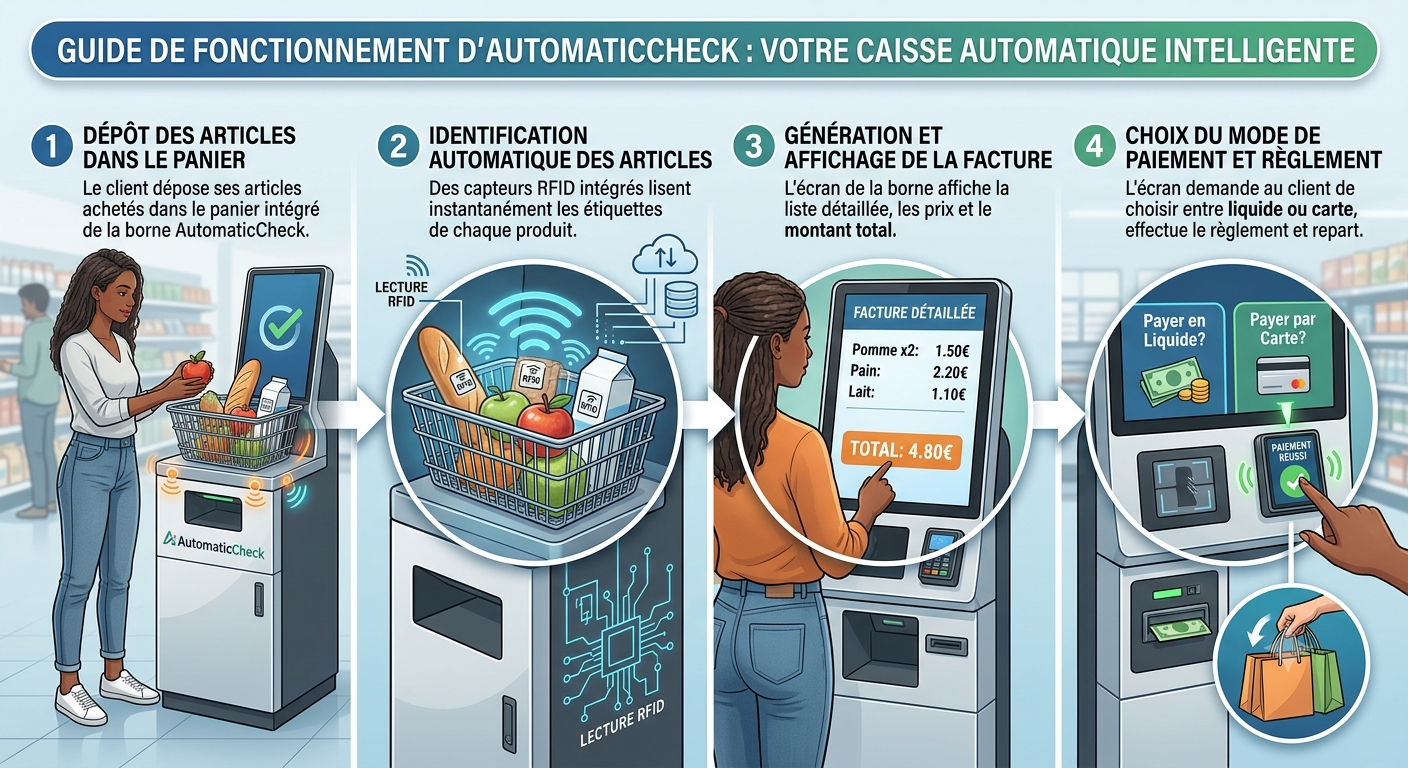
\includegraphics[width=\linewidth, height=0.84\textheight,
    keepaspectratio]{fonctionnement.png}
\end{frame}

%%═══════════════════════════════════════════════════════════════════════════
%% PARTIE 4 — MATURITÉ
%%═══════════════════════════════════════════════════════════════════════════

\begin{frame}{Niveau de maturité du projet}
  \vspace{-0.1cm}
  \centering
  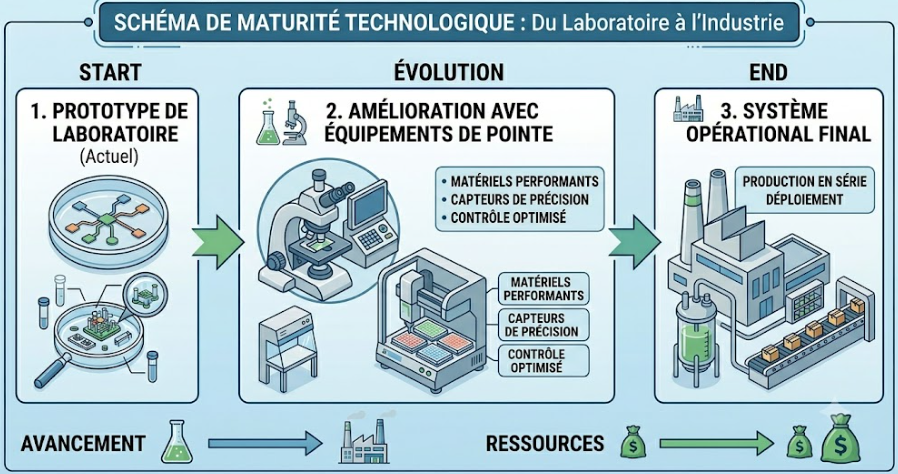
\includegraphics[width=\linewidth, height=0.84\textheight,
    keepaspectratio]{evolution.png}
\end{frame}

%%═══════════════════════════════════════════════════════════════════════════
%% PARTIE 5 — PERSPECTIVES
%%═══════════════════════════════════════════════════════════════════════════

\begin{frame}[shrink=5]{Perspectives — Les prochaines étapes}

  \vspace{0.25cm}

  \begin{tikzpicture}

    %% ── Carte 1 : Équipements de pointe ──────────────────────────────────
    \fill[acBlue, rounded corners=6pt]        (0,    2.6cm) rectangle (6.8cm, 5.4cm);
    \fill[white, opacity=0.12, rounded corners=4pt] (0.15cm, 4.6cm) rectangle (6.65cm, 5.25cm);
    \node[text=acGold, font=\fontsize{20}{20}] at (1.0cm, 4.92cm) {\faMicrochip};
    \node[text=white, font=\bfseries\small, anchor=west] at (1.6cm, 4.92cm)
      {Équipements de pointe};
    \node[text=white!85, font=\scriptsize, text width=6.2cm, align=left]
      at (3.4cm, 3.75cm)
      {Remplacement des composants actuels par du matériel
       haute performance : lecteurs RFID industriels, capteurs
       de précision et Raspberry Pi CM4 pour un contrôle
       optimisé en environnement commercial réel.};

    %% ── Carte 2 : Interface mobile ───────────────────────────────────────
    \fill[acLightBlue, rounded corners=6pt]   (7.2cm, 2.6cm) rectangle (14cm,  5.4cm);
    \fill[white, opacity=0.12, rounded corners=4pt] (7.35cm, 4.6cm) rectangle (13.85cm, 5.25cm);
    \node[text=white, font=\fontsize{20}{20}] at (8.2cm, 4.92cm) {\faMobile};
    \node[text=white, font=\bfseries\small, anchor=west] at (8.8cm, 4.92cm)
      {Interface mobile};
    \node[text=white!85, font=\scriptsize, text width=6.2cm, align=left]
      at (10.6cm, 3.75cm)
      {Développement d'une application mobile permettant
       au client de suivre sa facture en temps réel, de
       gérer ses achats et de recevoir ses reçus
       numériquement sur son smartphone.};

    %% ── Carte 3 : Gestion commerciale ────────────────────────────────────
    \fill[acGold, rounded corners=6pt]        (0,    0cm)    rectangle (6.8cm, 2.3cm);
    \fill[white, opacity=0.15, rounded corners=4pt] (0.15cm, 1.3cm) rectangle (6.65cm, 1.95cm);
    \node[text=white, font=\fontsize{18}{18}] at (1.0cm, 1.62cm) {\faChartBar};
    \node[text=white, font=\bfseries\small, anchor=west] at (1.6cm, 1.62cm)
      {Gestion commerciale intégrée};
    \node[text=white!90, font=\scriptsize, text width=6.2cm, align=left]
      at (3.4cm, 0.62cm)
      {Module de gestion des stocks, rapports de vente,
       alertes de réapprovisionnement et tableau de bord
       analytique pour les commerçants.};

    %% ── Carte 4 : APIs de paiement ───────────────────────────────────────
    \fill[acGreen, rounded corners=6pt]       (7.2cm, 0cm)   rectangle (14cm,  2.3cm);
    \fill[white, opacity=0.15, rounded corners=4pt] (7.35cm, 1.3cm) rectangle (13.85cm, 1.95cm);
    \node[text=white, font=\fontsize{18}{18}] at (8.2cm, 1.62cm) {\faCreditCard};
    \node[text=white, font=\bfseries\small, anchor=west] at (8.8cm, 1.62cm)
      {APIs de paiement};
    \node[text=white!90, font=\scriptsize, text width=6.2cm, align=left]
      at (10.6cm, 0.62cm)
      {Intégration des passerelles Mobile Money (MTN, Moov),
       Visa/Mastercard et solutions de paiement locales
       pour un règlement 100\,\% numérique.};

  \end{tikzpicture}

\end{frame}

%%═══════════════════════════════════════════════════════════════════════════
%% CONCLUSION
%%═══════════════════════════════════════════════════════════════════════════

\begin{frame}[shrink=5]{Conclusion}

  \vspace{0.2cm}
  \begin{columns}[t]
    \column{0.48\textwidth}

      \begin{block}{\faCheckCircle\enspace Ce que nous avons}
        \vspace{0.1cm}
        \begin{itemize}\setlength\itemsep{0.15cm}
          \item Un \textbf{prototype fonctionnel} validé en laboratoire
          \item Une identification RFID \textbf{opérationnelle}
          \item Une architecture logicielle \textbf{complète et ouverte}
          \item Un panier intelligent \textbf{imprimé en 3D}
        \end{itemize}
      \end{block}

      \vspace{0.25cm}
      \begin{block}{\faRocket\enspace Ce que nous visons}
        \vspace{0.1cm}
        \begin{itemize}\setlength\itemsep{0.15cm}
          \item Équipements de pointe \& interface mobile
          \item Gestion commerciale intégrée
          \item APIs de paiement multi-canal
          \item Déploiement dans les commerces béninois
        \end{itemize}
      \end{block}

    \column{0.48\textwidth}

      \begin{tikzpicture}
        \fill[acBlue, rounded corners=6pt] (0, 2.8cm) rectangle (6.5cm, 5.2cm);
        \node[text=acGold, font=\fontsize{28}{28}] at (3.25cm, 4.5cm)
          {\faLightbulb};
        \node[text=white, font=\bfseries\normalsize, text width=5.8cm, align=center]
          at (3.25cm, 3.5cm)
          {automaticCHECK : la réponse\\africaine à un problème africain};

        \fill[acGold, rounded corners=6pt] (0, 0cm) rectangle (6.5cm, 2.5cm);
        \node[text=acBlue, font=\bfseries\small, text width=5.8cm, align=center]
          at (3.25cm, 1.88cm) {\faHandshake\enspace Cherchons};
        \node[text=acBlue, font=\scriptsize, text width=5.8cm, align=center]
          at (3.25cm, 1.1cm)
          {Partenaires industriels · Investisseurs\\
           Distributeurs locaux · Pilotes commerciaux};
        \node[text=acBlue!60, font=\tiny\itshape]
          at (3.25cm, 0.3cm) {adebissi.niyi@gmail.com};
      \end{tikzpicture}

  \end{columns}

\end{frame}

%%═══════════════════════════════════════════════════════════════════════════
%% SLIDE MERCI
%%═══════════════════════════════════════════════════════════════════════════

{
\setbeamertemplate{footline}{}
\begin{frame}[plain]
  \begin{tikzpicture}[remember picture, overlay]
    \fill[acBlue] (current page.south west) rectangle (current page.north east);
    \fill[acGold] (current page.south west)
      rectangle ([yshift=0.15cm]current page.south east);
    \fill[acLightBlue!35!acBlue]
      ([xshift=0.55\paperwidth]current page.south west)
      rectangle (current page.north east);
    \fill[white, opacity=0.05]
      ([xshift=0.8\paperwidth, yshift=0.5\paperheight]current page.south west)
      circle (4cm);
    \node[text=white, opacity=0.15, font=\fontsize{110}{110}]
      at ([xshift=0.82\paperwidth, yshift=0.5\paperheight]current page.south west)
      {\faShoppingBasket};
    %% Merci
    \node[text=white, font=\fontsize{42}{46}\bfseries]
      at ([yshift=0.8cm]current page.center)
      {Merci pour votre attention};
    \node[text=acGold, font=\Large\bfseries]
      at ([yshift=-0.5cm]current page.center)
      {automatic\textcolor{white}{CHECK}};
    %% Sous-titre
    \node[text=white!70, font=\small\itshape]
      at ([yshift=-1.5cm]current page.center)
      {La caisse automatique intelligente pour le commerce africain};
    %% Présentateur
    \node[text=white!55, font=\footnotesize]
      at ([yshift=-2.4cm]current page.center)
      {Luc DJETO $\cdot$ Porteur : Sara Houéfa ADJAHO $\cdot$ Avril 2026};
  \end{tikzpicture}
\end{frame}
}

\end{document}
